\documentclass{article}
\usepackage[utf8]{inputenc}

\title{Blockchain for manufacturing \\
 A practice for using blockchain on ESP32 microprocessor}
\author{WANG, Yuqiang \\ PANG, Sui}
\date{December 2017}

\usepackage{natbib, graphicx, csquotes, epigraph, listings, url, textcomp, gensymb}
\usepackage{amsmath,geometry,amscd,amssymb,verbatim,enumerate,mathrsfs,graphicx,CJKutf8,color,scalerel,stackengine,xcolor,polynom, geometry}
\usepackage{float, subcaption}
\DeclareGraphicsExtensions{.png}
\renewcommand{\familydefault}{\rmdefault}

\begin{document}

\maketitle

\section{Introduction}
    The blockchain is a distributed database that maintains a continual growing list of records called blocks secured from tampering and revision. \citep{narayanan2016bitcoin} Previous summary to implement the blockchain technology in the Internet of Things is extensively analyzed. \citep{christidis2016blockchains} for  Adding on top of cryptographic principles and technics including zero-knowledge proof, we have seen a few opportunities in the industrial robot industry.

    In the automation industry of Japan and Europe, only two parties are involved in building an assembly line, the industrial robot companies who seal the robots, and the manufacturing companies who use them. However, the industry is less monopolized in China, and there usually multiple parties involved, and figuring out responsibility in a malfunction situation is hard. If a manufacturing company purchases the mechanical robot arm body and the electrical controller from separate companies.

    For instance, the robot arm from Capek Robotics and the electrical controller from Googol Tech, when malfunctions occur, it is hard to analysis if it is a mechanical, electrical, or software error. In a situation like this, the raw data from the robot sensors are required for analysis to determine the reliability, yet the manufacturing company was willing to offer or analysis these data, worrying a leak on the critical manufacturing process. The manufacturing company will usually blame the controller company first, and ask the latter for compensation. At the same time, the controller supplier will worry if the data is tempered for more compensation. Hence a need is created for the controller supplier either to deploy a zero-knowledge proof to the manufacturing company that it is not their fault without showing them the method or to build a private chain network for sharing these data with a trusted record and a lower maintenance cost. Currently, most of the blockchain application we have seen are developed on commercial electronics. However, these electronics are not widely accepted in the industry for consideration on cost, power consumption, and electromagnetic compatibility. We used a computational limited microprocessor ESP32 to fit the need of the industry and deployed a blockchain for sharing information.

\section{Objective}
    In this project, we plan to design a blockchain in an embedded platform to update firmware in a distributed manner. Instead of getting the next firmware version from a central server, the embedded device will get a verified update from the broadcast of nearby nodes.

\section{Methodology}

    \subsection{Hardware Introduction}

    We choose the ESP32 microprocessor from Espressif Systems for its hardware level integration for SHA-256 function and common wireless communication protocols. The specification of the board is followed: \citep{espressifGithub}
    \begin{itemize}
      \item Xtensa Dual-core 32-bit microprocessor, running at 240MHz
      \item 448 KByte ROM
      \item 520 KByte SRAM
      \item 4 x 16MBytes Flash
      \item Bluetooth 4.2
      \item Wifi 802.11 n(2.4GHz)
      \item SHA, AES, RSA, RNG Accelerator
    \end{itemize}

    With all these hardware level support, each esp32 node can connect to wifi automatically and connect with its neighbor through AP or even Ethernet through some protocols. With a Bluetooth module, the esp32 node also can detect its physical neighbors when needed. In order to simplify our processing difficulty, we use a trustable development board of ESP32 named “ESP32 circle” bought from Taobao. \citep{whyengineer} The photo of this board is shown in Fig.  \ref{fig:esp_circle}:

    \begin{figure}[h!]
      \centering
      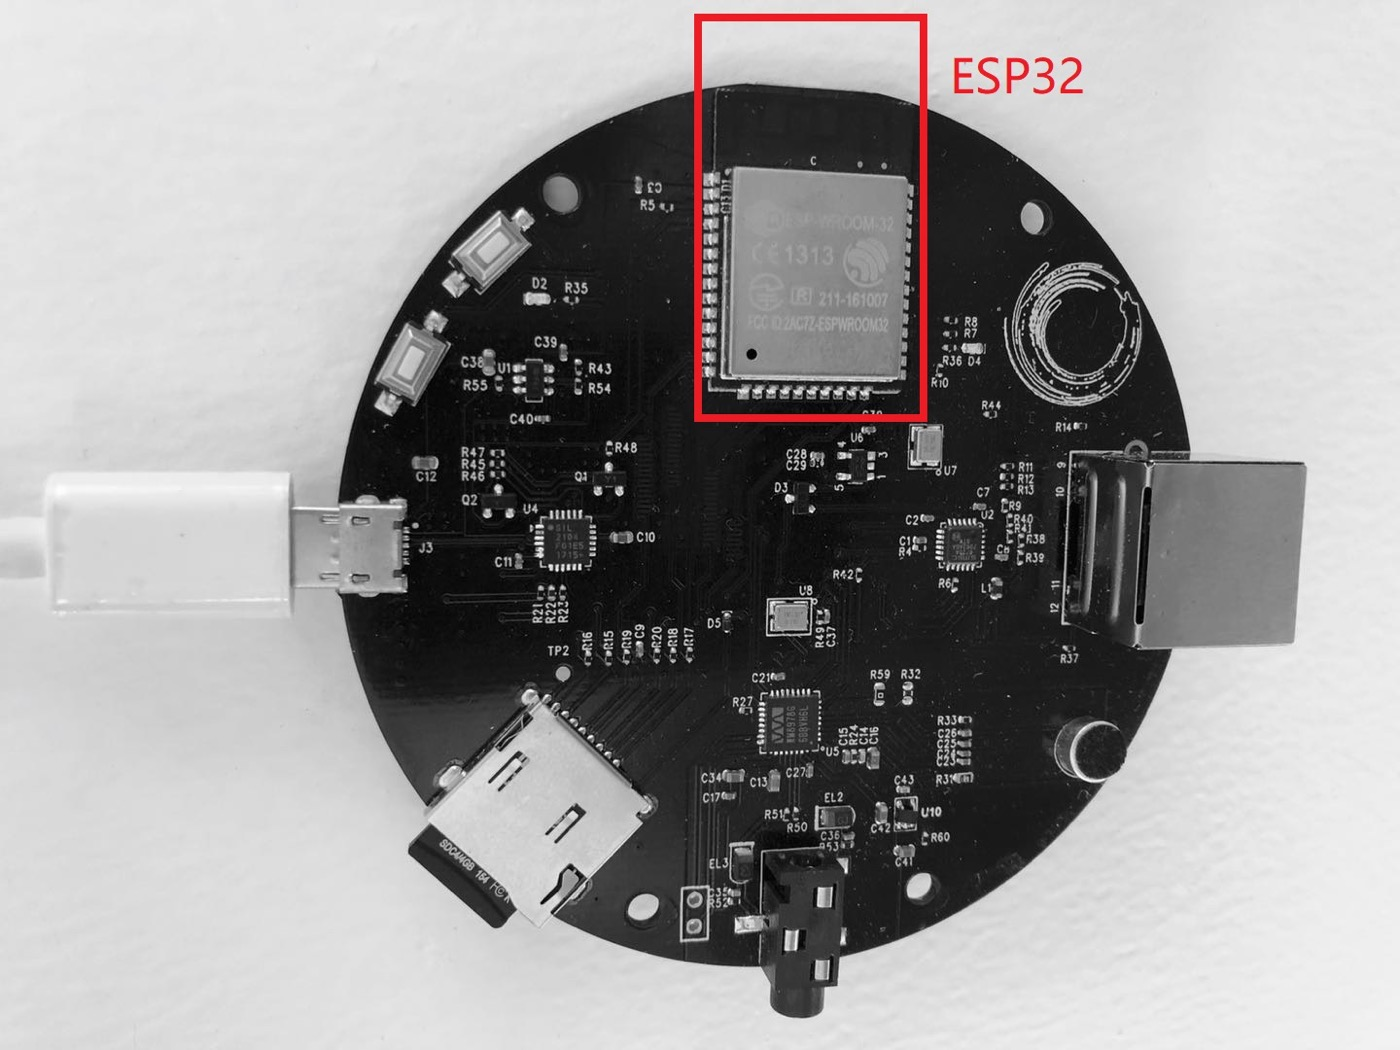
\includegraphics[scale=0.2]{esp32-circle.jpg}
      \caption{ESP32-circle module}
      \label{fig:esp_circle}
    \end{figure}

    The major four challenges we faced are the hashed blockchain data structure, the flash memory management, web server and HTTP requests, and over-the-air firmware flash. The first three challenges are the core blockchain problem, while the last one is a design choice for implementation and demonstration. To understand and implement the blockchain from an engineering perspective, we decide not to utilize an existing platform, but to build a blockchain from scratch. The blockchain we build are simplified and weak in scalability but have all the core functionality nonetheless.

    \subsection{Simple Blockchain Design}
        In order to establish this blockchain system, we designed a simple blockchain system without proof-of-work as our first version.

        //overall structure

        In this simple system, there is one special node (PC server) and more general node (ESP32). The function of the special node is providing new blocks, whole chain and the binary file (firmware) when requested by a general ESP32 node. The flow chat of ESP32 node:

        \subsubsection{Block Design}
        The block is stored in an array in fixed memory address with the following data structure:

        \subsubsection{JSON object}

        \begin{itemize}
          \item index
          \item timestamp
          \item the hash value of the .bin data
          \item the hash value of the previous block
          \item the hash value of the current block
        \end{itemize}

        The hash function we choose is SHA-256, a subclass of the Secure Hash Algorithm, a reliable hash function which is proved by Bitcoin system. We utilize the hardware SHA-256 solver on the ESP32 chip for non-blocking thread calculation. All items in the block are stored in the array of an 8-bit unsigned integer for the ease to integrate with the SHA-256 solver.

        \subsubsection{blocksize}
        \begin{figure}[h!]
          \centering
          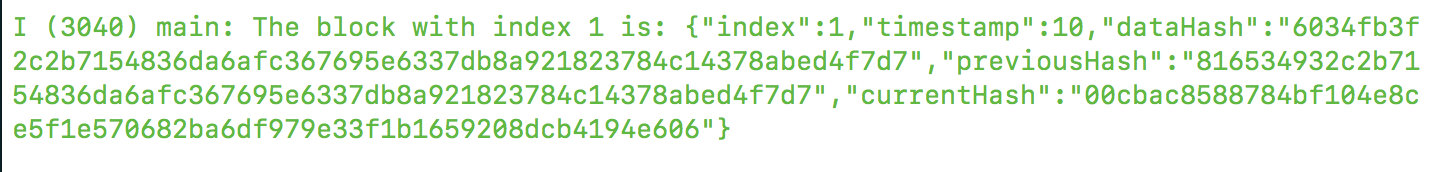
\includegraphics[scale=0.5]{lastest-block}
          \caption{screen shot of one block}
          \label{fig:lastest block}
        \end{figure}

      \subsubsection{flash memory management}
          //why use flash

          //how to use flash – by partition

          In order to store a small scale of array, the flash memory on chip is partitioned and utilized for data management. The partition table on the chip is hand crafted, and can be simplified to four partitions:
          \begin{itemize}
            \item unchangeable kernel and over-the-air function
            \item changeable, verified, running applications
            \item verified blockchain and the application file waiting to be flashed
            \item unverified new blocks
          \end{itemize}

          For the demonstration purpose, all flash memory sizes are fixed.

          \begin{figure}[h!]
            \centering
            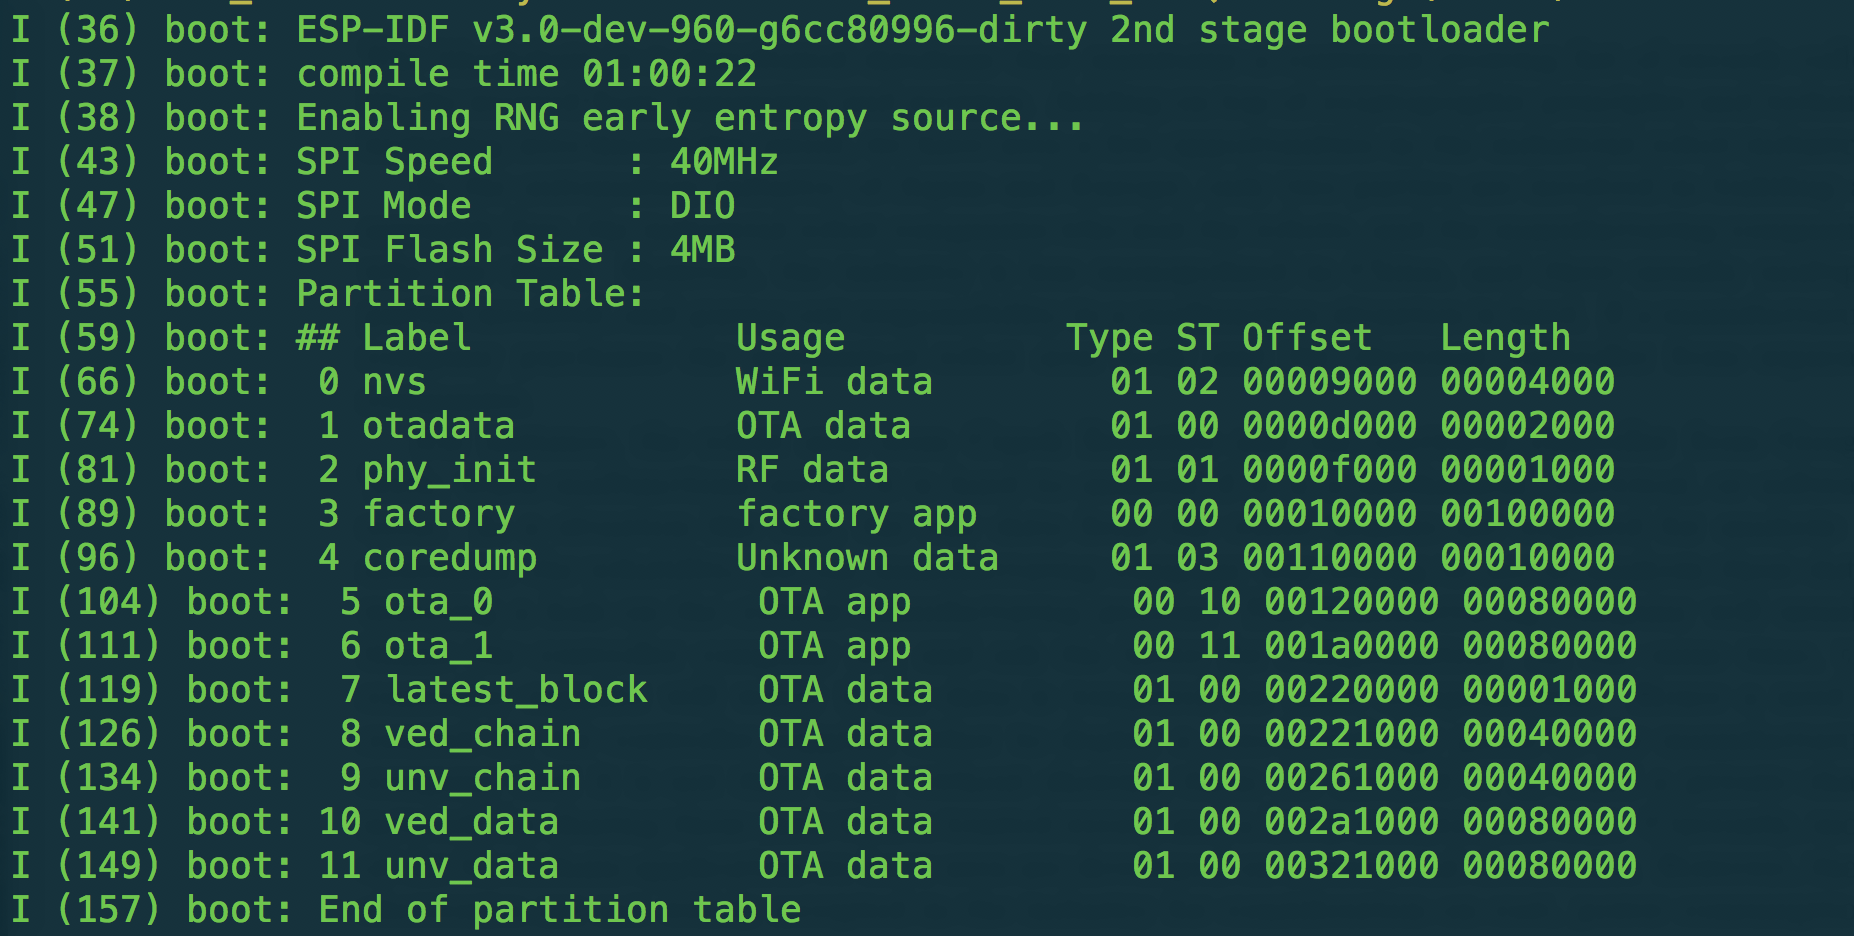
\includegraphics[scale=0.1]{partitionTable}
            \caption{screen shot of the complete partition table}
            \label{fig:partition table}
          \end{figure}

          // introduce the usage of every partition and why the design like this?

          //why there is a latest block partition

          //why unv chain and unv data

          //how to store the blockchain and how to find the whole chain by the latest block


      \subsubsection{validation}
          //how to get current hash
          //how to verify the whole chain in flash
          //how to verify the data file

    \subsection{web server and http requests}
        A simple web server with hardcoded IP address is written to the chip for access the upcoming data. The data are transmitted through web socket in JSON format.
        // socket
        //HTTP protocol
        //request part
        //web server part

    \subsection{over-the-air firmware flash}
        //OTA structure and how it works when updating

        The verified application binary will be flashed on board in an over-the-air process.

\section{Experimental evaluation}
    \subsection{block structure}
    \subsection{verify functions}
    \subsection{latest block chain, chain, and binary data store}
    \subsection{HTTP web server in PC node}
    \subsection{HTTP request in ESP32 node}
    \subsection{HTTP web server in ESP32 node}

\section{Future Plan}
    \subsection{combine}
    \subsection{over-the-air firmware flash}
    \subsection{neighbor node list}
    \subsection{Ethernet connect}
    \subsection{TF card for storage}
    \subsection{zero proof of work to make the system safe}

\section{Analysis}
    \subsection{Limitation}

\section{Conclusion}
    It is an interesting project, but much more difficult than our first think. Did a lot and learned a lot.


\bibliographystyle{plain}
\bibliography{references}
\end{document}
